\section{中心极限定理与 Gaussian 近似}
\label{sec:05-Probability/08-Limit-Theorems/03}

一次 A/B 实验跑完了。对照组 5000 人，转化率 \(10.0\%\)；实验组 5000 人，转化率 \(11.0\%\)。产品经理问：这一个百分点，是新功能起作用了，还是随机波动？

上一节的大数定律在这里帮不上忙。它只承诺样本量足够大时转化率会靠近真值，却没有给出``足够大''的刻度，也没说清什么幅度的差距算正常。要回答这个问题，你需要的不是均值的位置，而是均值周围那圈波动的形状与尺寸。

中心极限定理提供的正是这个。它管的是波动的形状，不是均值的位置——这两件事经常被混为一谈，混淆之后得到的结论往往比不做推断更危险。

\subsection{把塌缩的信息重新拉开}

设 \(X_1,X_2,\ldots\) 独立同分布，\(\E[X_i]=\mu\)，\(0<\Var(X_i)=\sigma^2<\infty\)。大数定律说 \(\bar X_n-\mu\to0\)：差值本身塌进一个点，所有分布信息被压没了。

如果在压缩之前先把差值放大呢？上一节末尾算过，\(\bar X_n-\mu\) 的典型尺度是 \(\sigma/\sqrt n\)。乘上 \(\sqrt n\) 恰好抵消这个衰减，被压扁的信息就会重新舒展开，露出一个不退化的形状：
\[
\frac{\sqrt n\,(\bar X_n-\mu)}{\sigma}\xrightarrow{d}\mathcal N(0,1).
\]
等价地写成日常使用的样子，
\[
\bar X_n\;\approx\;\mathcal N\!\left(\mu,\ \frac{\sigma^2}{n}\right),
\]
其中的 \(\approx\) 指标准化之后的分布函数与标准正态的分布函数差距很小，而不是说两边相等——两边其实都随 \(n\to\infty\) 塌向 \(\mu\)，近似说的是塌缩之前的形状。

放大倍数没有第二个选择。用 \(n^{0.4}\) 放大，波动仍被压向零，极限退化成常数；用 \(n^{0.6}\)，波动被放大到发散，没有极限分布。独立和的标准差按 \(\sqrt n\) 增长而均值按 \(n\) 增长，二者的比值以 \(1/\sqrt n\) 衰减，\(\sqrt n\) 是唯一能让分布信息活下来的标度。

顺手澄清一个流传很广的说法：``数据多了就会变正态。''不对。原始 \(X_i\) 的分布一点没变，Bernoulli 变量到了 \(n=10^6\) 仍然只取 \(0\) 和 \(1\)。趋近钟形的是标准化和这个构造出来的统计量，不是数据本身。看直方图判断``我的数据正态吗''，与中心极限定理无关。

\begin{center}
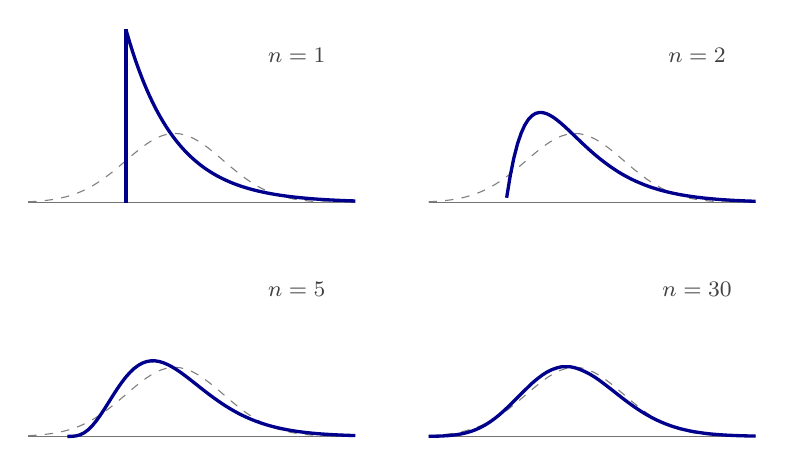
\begin{tikzpicture}[x=0.62cm,y=2.2cm,font=\footnotesize]
  \begin{scope}
    \draw[black!55] (-3,0) -- (3.7,0);
    \draw[dashed,black!50] plot[domain=-3:3.7,samples=70] (\x,{0.3989*exp(-\x*\x/2)});
    \draw[very thick,blue!55!black] (-1,0) -- (-1,1);
    \draw[very thick,blue!55!black] plot[domain=-0.995:3.7,samples=70] (\x,{exp(-(\x+1))});
    \node[black!75] at (2.5,0.85) {\(n=1\)};
  \end{scope}
  \begin{scope}[shift={(8.2,0)}]
    \draw[black!55] (-3,0) -- (3.7,0);
    \draw[dashed,black!50] plot[domain=-3:3.7,samples=70] (\x,{0.3989*exp(-\x*\x/2)});
    \draw[very thick,blue!55!black] plot[domain=-1.4:3.7,samples=70]
      (\x,{1.41421*(2+1.41421*\x)*exp(-(2+1.41421*\x))});
    \node[black!75] at (2.5,0.85) {\(n=2\)};
  \end{scope}
  \begin{scope}[shift={(0,-1.35)}]
    \draw[black!55] (-3,0) -- (3.7,0);
    \draw[dashed,black!50] plot[domain=-3:3.7,samples=70] (\x,{0.3989*exp(-\x*\x/2)});
    \draw[very thick,blue!55!black] plot[domain=-2.2:3.7,samples=70]
      (\x,{exp(4*ln(5+2.23607*\x)-(5+2.23607*\x)-2.3734)});
    \node[black!75] at (2.5,0.85) {\(n=5\)};
  \end{scope}
  \begin{scope}[shift={(8.2,-1.35)}]
    \draw[black!55] (-3,0) -- (3.7,0);
    \draw[dashed,black!50] plot[domain=-3:3.7,samples=70] (\x,{0.3989*exp(-\x*\x/2)});
    \draw[very thick,blue!55!black] plot[domain=-3:3.7,samples=70]
      (\x,{exp(29*ln(30+5.47723*\x)-(30+5.47723*\x)-69.5565)});
    \node[black!75] at (2.5,0.85) {\(n=30\)};
  \end{scope}
\end{tikzpicture}

\emph{起点故意选了不对称的指数分布：\(n=1\) 时密度在左端顶到最高再单调下滑，毫无钟形可言。粗线是 \(n\) 个样本标准化均值的真实密度，虚线是标准正态。\(n=5\) 已初具形状，\(n=30\) 的中段几乎重合——但右尾那一截仍然压不下去，这是下面要单独算的账。}
\end{center}

\subsection{三根支柱，抽掉哪根会怎样}

经典版本要求独立、同分布、方差有限。逐条看它们各自挡住什么。

方差有限是最硬的一根。Cauchy 分布连均值都没有，标准化无从谈起，独立同分布 Cauchy 的平均还是 Cauchy。但边界并不是一堵墙，而是一片过渡带：独立和的可能极限构成稳定分布族，特征函数形如 \(\exp(-c\abs t^\alpha)\)（对称情形），尾指数 \(\alpha\in(0,2]\) 决定尾巴的厚薄。Gaussian 是 \(\alpha=2\) 的成员，也是这个家族里唯一方差有限的成员；Cauchy 是 \(\alpha=1\)。当 \(\alpha\) 从 \(2\) 降到 \(1.8\)、\(1.5\)，极限分布的尾部依次变厚，大偏差的概率质量依次加重。所以在重尾数据上硬套正态置信区间，得到的区间不是稍微窄了一点，而是错了一个族。

同分布这一根可以放松。分布各异时，只要满足 Lindeberg 条件——粗略说，没有任何单个变量对总方差的贡献占比过高——标准化和仍趋于正态。写出来是
\[
\frac1{s_n^2}\sum_{i=1}^n\E\bigl[(X_i-\mu_i)^2\ind_{\set{\abs{X_i-\mu_i}>\varepsilon s_n}}\bigr]\to0,
\qquad s_n^2=\sum_i\Var(X_i).
\]
它排除的病态很具体：若第 \(n\) 个变量的方差是 \(2^n\) 而前面都是 \(1\)，总和完全由最后一个变量的一次实现决定，钟形自然出不来。数据工作里对应的是``少数几个巨型用户贡献了绝大部分流量''，这时对总量做正态推断是不成立的。

独立这一根同样可以放松成弱依赖，但极限方差要改。相邻观测相关时，极限方差不再是边缘方差，而是长期方差
\[
\sigma^2_{\text{long}}=\Var(X_1)+2\sum_{k\ge1}\Cov(X_1,X_{1+k}),
\]
正相关会把它抬高。会话内的多次点击、同一用户的重复请求、时间序列上的惯性都属于这一类。忽略这一项而按独立公式算标准误，区间会系统性偏窄，显著性会系统性虚高——这是线上实验里最常见的一种自欺。

\subsection{收敛有多快：\texorpdfstring{\(1/\sqrt n\)}{1/sqrt n}，而且尾部最慢}

极限陈述不告诉你 \(n\) 多大才够。Berry--Esseen 定理补上了速率：若三阶绝对中心矩 \(\rho=\E[\abs{X-\mu}^3]\) 有限，令 \(Z_n=\sqrt n(\bar X_n-\mu)/\sigma\)，则对所有 \(x\) 一致地
\[
\bigl|F_{Z_n}(x)-\Phi(x)\bigr|\le\frac{C\rho}{\sigma^3\sqrt n},
\]
其中 \(C\) 是与分布无关的常数（目前已知的上界约 \(0.4748\)）。

这个界有两个使用要点。第一，\(1/\sqrt n\) 是分布函数的一致误差，比大数定律那种逐点概率的 \(1/n\) 慢一档，因为要求强得多。第二，也是更实用的一点，系数 \(\rho/\sigma^3\) 是标准化偏度的度量：Bernoulli\((0.5)\) 对称，这个比值是 \(0.5\)，\(n\) 不大时正态近似就很好；率为 \(1\) 的指数分布，比值约 \(2.4\)，同样的 \(n\) 误差大好几倍；三阶矩都不存在的重尾分布，这条定理连前提都不满足，你连速率保证都没有。

于是``\(n\ge30\) 就可以放心用正态近似''是一句伪命题。\(n\) 不是唯一变量，偏度和尾部厚度同等重要。

更要紧的是，Berry--Esseen 给的是全轴上的最大误差，而这个误差在实践中主要花在了尾部——偏偏尾部才是你关心的地方。置信区间取 \(95\%\) 或 \(99\%\) 分位，假设检验看的是 \(p\) 值，这些量全都由尾部决定。

\begin{center}
\begin{tikzpicture}[x=2.2cm,y=1.05cm,font=\footnotesize]
  \draw[black!45] (1.5,-4.2) rectangle (4.2,-0.7);
  \foreach \y in {-1,-2,-3,-4}{\draw[black!45] (1.5,\y) -- (1.62,\y);
    \node[left,black!70] at (1.5,\y) {\(10^{\y}\)};}
  \foreach \x in {2,3,4}{\draw[black!45] (\x,-4.2) -- (\x,-4.08);
    \node[below,black!70] at (\x,-4.2) {\(\x\)};}
  \begin{scope}
    \clip (1.5,-4.2) rectangle (4.2,-0.7);
    \draw[dashed,thick,black!60] plot[domain=1.5:4.25,samples=60] (\x,{-0.399-0.2171*\x*\x});
    \draw[very thick,blue!55!black] plot[domain=1.5:4.25,samples=60]
      (\x,{(29*ln(30+5.47723*\x)-(30+5.47723*\x)-69.5565)/2.302585});
  \end{scope}
  \node[right,black!70] at (4.22,-2.9) {真实右尾（\(n=30\)）};
  \node[right,black!70] at (4.22,-3.75) {正态近似};
  \node[below,black!70] at (2.85,-4.62) {标准化偏差 \(z\)};
\end{tikzpicture}

\emph{同一组 \(n=30\)、上图中段已经几乎重合的曲线，把右尾放到对数刻度上看：\(z=2\) 附近两条线还贴着，到 \(z=4\) 时真实密度已是正态近似的七倍左右。中心区域拟合得好，不代表你报告的 \(p\) 值可信。}
\end{center}

判断能不能信，有一条粗糙但好用的规则：看你要用的分位点落在分布的哪个位置。中位数附近的推断，中心极限定理很宽容；\(99.9\%\) 分位或者尾部概率的估计，就要么加大 \(n\)，要么改用 bootstrap、精确检验，要么直接对尾部建模（见\hyperref[sec:05-Probability/06-Common-Distributions/08]{``极值分布与尾部风险''}）。二项分布也有同一条经验规则的具体版本：\(np\) 与 \(n(1-p)\) 都不宜太小。\(p=0.01\)、\(n=100\) 时 \(\mu=1\) 而 \(\sigma\approx1\)，分布几乎全部质量堆在 \(0\) 和 \(1\) 两点上，拿一条向左延伸到负无穷的对称钟形去套，尾部误差可以大到没有意义。

\subsection{回到那一个百分点}

现在可以回答开头的问题了。两组转化率之差 \(\hat p_B-\hat p_A=0.01\)，中心极限定理说这个差近似正态，方差约为
\[
\frac{\hat p_A(1-\hat p_A)}{n_A}+\frac{\hat p_B(1-\hat p_B)}{n_B}
=\frac{0.1\times0.9}{5000}+\frac{0.11\times0.89}{5000}\approx3.76\times10^{-5},
\]
标准误约 \(0.0061\)。观测到的差是标准误的 \(1.63\) 倍，双侧 \(p\) 值约 \(0.10\)——按常规阈值不显著。若想让同样大小的真实效应达到显著，每组样本量需要提到七千二百左右（把标准误压到 \(0.0051\) 以下）。

注意这套推断从头到尾没有用到点击行为的任何分布细节。输入只有样本量、样本均值和样本方差，输出是 \(p\) 值和置信区间。民意调查报告的``误差范围 \(\pm3\%\)''是同一台机器的产物：\(1.96\times\sqrt{0.25/1000}\approx0.031\)；质量控制图上的 \(\mu\pm3\sigma/\sqrt m\) 也是。现代统计推断的基础设施几乎整个架在这一条定理上。

为此叠了三层近似，每一层都可能出问题。第一层是分布近似，误差由 Berry--Esseen 以 \(O(1/\sqrt n)\) 控制，尾部尤其吃紧。第二层是用 \(\hat\sigma\) 顶替未知的 \(\sigma\)，Slutsky 定理保证极限分布不变——用到的正是上一节讲的``依分布收敛与依概率收敛到常数可以拼接''。第三层最隐蔽：把渐近结果当成有限样本结果用，\(95\%\) 的覆盖率其实只是渐近的，小样本下 \(t\) 分布给出的区间更宽，宽出来的部分正是为估计 \(\sigma\) 付的钱。

那么这条定理本身怎么证？形状从原始分布里彻底消失了，无论起点是均匀、Bernoulli 还是指数，终点都是同一条曲线，这件事靠 Chebyshev 那样的矩估计是压不出来的。下一节换一套工具：把分布编码成一个函数，让独立求和变成函数相乘，剩下的事就交给微积分里那个熟悉的 \((1+x/n)^n\)。
